%% from aastex61.cls with a few tweaks to allow for the unique format required.
\documentclass{rnaastex}

\begin{document}

\title{Line broadening from spectral channel width and a response function}

%% Note that the corresponding author command and emails has to come
%% before everything else. Also place all the emails in the \email
%% command instead of using multiple \email calls.
\correspondingauthor{Eric Koch}
\email{ekoch@ualberta.ca}
\author[0000-0001-9605-780X]{Eric Koch}
\author[0000-0002-5204-2259]{Erik Rosolowsky}
\affiliation{University of Alberta, Department of Physics 4-183 CCIS, Edmonton AB T6G 2E1, Canada}

\author{Adam Leroy}
\affiliation{The Ohio State University, Department of Astronomy, 140 West 18th Avenue, Columbus, OH 43210, USA}


%% Note that RNAAS manuscripts DO NOT have abstracts.
%% See the online documentation for the full list of available subject
%% keywords and the rules for their use.
\keywords{}

%% Start the main body of the article. If no sections in the
%% research note leave the \section call blank to make the title.

\section{}

% - Intro: define the domain (radio), the technology (correlation spectrometers), and the problem (<~2 channels across a line)

Observations of spectral-lines are affected by systematic line broadening from the spectral response function of the telescope's spectrometer. Although analyses in the radio and submillimetre often incorrectly assume a spectral response of independent, top-hat channels, the spectral response function is a combination of instrumentation and signal processing, just like at other wavelengths.  Since typical observing strategies resolve lines with only a few channels ($\sim3\mbox{--}5$ per full-width-half-max), spectral-line properties will be biased---including accurate line width measurements--- without accounting for the spectral response.  In this note, we compare different methods for inferring the line width of a single noiseless Gaussian.  We explore how biased the line width estimates are when not accounting for the spectral response and show that typically-used correction factors from the literature do not correctly remove this bias.

% - Define a data model: Gaussian, noiseless, perfect channel model, empirical correlation basis (Leroy+2016) and convolution kernel.  I think you could maybe drop the current equation 1 and just describe it as a boxcar smoothing and sampling. 

We consider a single noiseless Gaussian as the simplest model. When sampled by an ideal spectrometer, where each channel is independent, the Gaussian model is smoothed with a top-hat kernel with a width equal to a spectral channel.  The value measured in each channel is the weighted average of the Gaussian over the channel width. Compared to the original Gaussian, the observed spectrum has a lower amplitude and larger $\sigma$.  This effect becomes more extreme as $\Delta v \rightarrow \sigma$.

% Spectral-lines measured by an ideal spectrometer\footnote{Each channel is independent of each other.} are a weighted average of the line profile over the finite spectral channel. A Gaussian centered at velocity $\mu$ with an amplitude of $A$ and width of $\sigma$ that is averaged over channels centered at $v$ with width $\Delta v$ has the form
% \begin{equation}
%     \label{eq:finite_gaussian}
%     G(v) = \frac{A}{(\Delta v)^2} \left[ {\rm erf}\left( \frac{\mu - (v - \Delta v / 2)}{\sqrt{2}\sigma} \right) - {\rm erf}\left( \frac{\mu - (v + \Delta v / 2)}{\sqrt{2}\sigma} \right) \right].
% \end{equation}
% Compared to the original Gaussian, the channel-averaged version $G(v)$ has lower amplitude and larger $\sigma$.  This effect becomes more extreme as $\Delta v \rightarrow \sigma$. 

Though independent, top-hat spectral channels are commonly assumed, real radio observations often have a more complex spectral response.
However, real spectrometers do not produce a perfect top-hat response function.  Signals measured by a spectrometer are truncated by some maximum time lag, which is set by XXX and whose inverse determines the spectral resolution.  This limit on the spectral resolution is equivalent to multiplying the signal by a top-hat function, the Fourier transform of which is a sinc function.  If the frequency of the measured signal is located at the centre of a spectral channel, the response is effectively a top-hat kernel.  However, frequencies offset from the channel centres will exhibit ringing due to the sinc-function.  Since all observed signal have a finite spectral width, this ringing effects all observations.  To reduce this ringing, spectrometers apply an apodizing function prior to correlating the input signal\footnote{e.g., \url{https://safe.nrao.edu/wiki/pub/Main/ALMAWindowFunctions/Note_on_Spectral_Response.pdf}}.  A Hann kernel is often used as an apodizing function, which minimizes spectral ringing while at the expense of correlating nearby channels.  For some radio and submillimetre instruments, the response function is well-charaxterized and can be included when modelling the observed spectra \citep{rosolowsky2008}.  In the absence of this information, or when an approximation can be used, a three-element Hann-like kernel ($[k, 1 - 2k, k]$, where $k$ is the channel coupling) that accounts for nearest-neighbour channel correlations can be used as an approximate spectral response function \citep{leroy2016}.

The top row of panels in Figure \ref{fig:width_recovery_comparison} show a Gaussian profile averaged over spectral channels and convolved by a Hann-like kernel ($k=0.11$) with channel widths ($\Delta$) equal to the Gaussian standard deviation ($\sigma$). Both an ideal top-hat and Hann-like kernel broaden the Gaussian profile, underestimating the amplitude and overestimating the line width.

% - Line positioning comment: centre vs edge matters (row 1 of figure)

These two panels also exhibit that the shape of the observed spectrum depends on how the line is positioned with respect to the spectral channels. The left panel shows the ideal case where the position of the peak lies at the channel centre and is minimally broadened by the spectral response.  The right panel shows the worst case of broadening from the spectral response: when the peak lies at the edge of two channels.  Since the peak location is a properties of the source, it cannot be known a priori.  Recovering the correct line properties thus requires accounting for the spectral response.

% For some instruments, the response function is well-characterized \citep{rosolowsky2008}, particularly for instruments whose response functions significantly alters the observed line shape \citep[e.g.][]{martin2015}.

% The line broadening can be forward-modelled by channel-averaging and convolving the fit model with the spectral response function prior to comparing with the observed spectrum. Forward-modelling of spectrum lines has been used for some radio observations \citep{rosolowsky2008} and is commonly used for shorter wavelength observations \citep[e.g.,][]{martin2015}.

% - How to measure line width: fits, fits with forward model, equivalent width, second moment.

To correctly recover the line properties, the spectral response can be included in the model fit to the observed line profile.  We forward-model the spectral response by averaging a Gaussian profile over the channel widths and convolving with a Hann-like kernel ($k=0.11$) prior to comparing with the observed profile.  We note that forward-modelling with an known (or approximate) spectral response function is common-practice in many fields \citep[e.g.,][]{martin2015}, but is used in only a few radio studies \citep{rosolowsky2008}.  In the noiseless case used here, this model is defined to recover the correct line properties.
% XXX We later show that forward-modelling recovers unbiased line properties in the presence of moderate noise.
% When fitting an analytical model, it is straightforward to forward-model the spectral response function, which can be approximated from the noise properties of the data \citep{leroy2016}. 

While forward-modelling correctly accounts for the spectral response, it requires directly fitting the spectrum, which can be computationally-expensive, requires knowing the correct model to fit to, and may be adversely affected by noise.  Instead, many studies use approximate methods for calculating the line width, usually assuming a Gaussian shape. We compare the forward-model fit with four other methods:
\begin{enumerate}
    \item {\bf Fit to Gaussian} without forward modelling.
    \item {\bf Moment 2}: $\sigma_{\rm Mom2}=\sqrt{\sum_i T_i (v_i - v_0)^2 / \sum_i T_i}$ where $T_i$ is the value at $v_i$ and $v_0$ is the centroid.
    \item {\bf Equivalent width}: $\sigma_{\rm equiv} = T_{\rm peak} / \sqrt{2\pi} \Sigma$ where $T_{\rm peak}$ is the measured amplitude and $\Sigma= \sum_i T_i \Delta v$ is the integrated intensity \citep{heyer2001,leroy2016,sun2018}.
    \item {\bf half-width-half-max (HWHM)} estimated from the locations where the observed spectrum is equal to half of the measured peak \citep{stilp2013a,stilp2013b,koch2018}.
\end{enumerate}

% - How to correct line width measurements: CPROPS ad hoc, Leroy+2016 kernel extension.  Can you link the two in the k=0 case and shorten this down?

When approximate line width methods or fitting without forward-modelling are used, many radio studies adopt a line width correction factor for a top-hat kernel.  The line broadening is assumed to equal the effective width from setting the area of a Gaussian equal to the rectangular area over one channel, which is then subtracted in quadrature from the measured line width \citep{cprops}.  To account for channel correlations, \citet{leroy2016} extended this correction factor with an empirical calibration.  \citet{leroy2016} characterize the typical channel-to-channel correlation ($r$) and fit a polynomial relating the channel coupling $k$ from a three-element Hann-like kernel ($[k, 1 - 2k, k]$) to $r$: $k\approx 0.0 + 0.47r - 0.23r^2 - 0.16r^3 + 0.43 r^4$. This empirical calibration gives a line broadening correction factor of:
\begin{equation}
    \label{eq:leroy16_corrfact}
    \sigma_{\rm chan} \approx \frac{\Delta v}{\sqrt{2\pi}} \left( 1.0 + 1.18k + 10.4 k^2 \right).
\end{equation}
As $k\rightarrow0$, the term in brackets approaches unity to the assumed correction factor of a top-hat response.  \citet{sun2018} give the channel correlations for a number of CO datasets of nearby galaxies. For the example here, we use $r=0.26$ ($k=0.11$) for the IRAM-30m CO(2-1) data of M33 \citep{druard2014}.
% Using this approximation for a response function, we convolve the channel-averaged Gaussian (Eq. \ref{eq:finite_gaussian}) in Figure \ref{fig:width_recovery_comparison} to show how a realistic response function further broadens the Gaussian.


% - Describe rows 2 and 3 of the figure.  Outline why we're stepping from one to the next.  As noted in the document, why the reduction in quality when k->0?

We generate a series of model spectra varying the sampling $\Delta v / \sigma$ to determine where the different line width methods correctly recover the line width. For each spectrum, we calculate the line width from each method, with and without subtracting a correction factor (Eq. \ref{eq:leroy16_corrfact}), for the channel-averaged Gaussian with independent channels (top-hat kernel) and channels correlated by a Hann-like kernel. The bottom four panels in Figure \ref{fig:width_recovery_comparison} show the measured line widths.

When the line is centered on a channel (first column), we find that the line width methods are similarly biased and convolving with a Hann-like kernel only increases the line broadening.  We subtract Eq. \ref{eq:leroy16_corrfact} in quadrature from the measured line widths and find that correction factor overestimates line broadening for independent channels ($k=0$) but correctly removes the line broadening to $<5\%$ when the channels are correlated ($k=0.11$) for $\sigma/\Delta v \geq 1$.

When the line is centered on the edge of a channel (second column), there is substantial deviation between the methods. With independent channels, the Gaussian fit and second moment are biased similarly to when the peak is centered on a channel, and applying Eq. \ref{eq:leroy16_corrfact} ($k=0$) also overestimates line broadening from a top-hat kernel.  The equivalent width and HWHM are biased to larger values than the latter methods because they depend on the amplitude of the profile, which is underestimated more than in the channel-centre case.  In this case, Eq. \ref{eq:leroy16_corrfact} ($k=0$) {\it underestimates} the line broadening. This discrepancy between methods suggests that, when a line is marginally resolved ($\sigma / \Delta v < 2$), methods that leverage information across many channels are vastly preferable over those that focus on the line core (equivalent width and HWHM).

When a Hann-like kernel is applied to lines at channel edge, the line widths are qualitatively the same as those with a top-hat kernel.  Equation \ref{eq:leroy16_corrfact} ($k=0.11$) works well for the Gaussian fit and second moment for $\sigma/\Delta v \geq 1$, but underestimates the line broadening for the equivalent width and HWHM.

It is curious that Eq. \ref{eq:leroy16_corrfact} only corrects for line broadening when $k\gt0$.  This discrepancy results from Eq. \ref{eq:leroy16_corrfact} being empirically-calibrated from real observations assuming the response function is a Hann-like kernel.  Thus it is calibrated to work for this case.  As $k\rightarrow0$, there is a transition to the response of a top-hat kernel only.  Since the $k=0$ case does not correctly account for line broadening in any of the tested cases, the prefix of $\frac{\Delta v}{\sqrt{2\pi}}$ is the incorrect line width contribution for a top-hat kernel (i.e. independent channels).
% While most observational data will have correlated channels and can be treated in the $k\gt0$, the $k=0$ case may result when the data are severely under-sampled to reduce the noise. XXX

% XXX Mention maximum uncertainty from channel edge vs. expected uncertainties from randomly centering the line within a channel XXX.
% The examples shown here demonstrate the best (channel centre) and worst (channel edge) cases of recovering spectral properties.  Assuming that

% - Recommendations:
    % - More channels across lines plz.
    % - Otherwise: fit or second moment is preferred for single Gaussians.  Must use correction that accounts for channel correlation.

When using approximate methods to find the line width, our results indicate that: 
\begin{enumerate}
    \item When channels are correlated by a Hann-like kernel ($k=0.11$), the channel width required for the the measured line width to deviate by $<5\%$ from the actual line width is $\sigma / \Delta v \geq 2$ for fitting a Gaussian and the second moment and $\sigma / \Delta v \geq 4$ for the equivalent width and HWHM.  Assuming that, for most observational data, deviations of $<5\%$ are smaller than the uncertainty from noise, there is no need to account for line broadening above these limits.  Where possible, we recommend that observational setups sample $\sigma / \Delta v > 2$ (or $5$ channels per FWHM).
    \item When fitting an analytical model to observed data, it is vastly preferable to forward-model with a spectral response function.
    \item Methods that estimate the line width with information over multiple channels (fitting, second moment) are preferable over those that use only the line core (equivalent width, HWHM). These latter methods can place upper limits on the line width, but should be treated with caution when $\sigma / \Delta v <4$.
    \item A spectral response function that is more complex than a top-hat kernel needs to be accounted for.  In the example shown here, the Hann-like kernel increased measured line widths by $\sim10\%$ compared to the top-hat kernel.
\end{enumerate}

We stress that these recommendations are only for {\it high signal-to-noise, single Gaussian spectra}; multi-component spectra will change the biases for these methods.  We also note that each of the methods will break down for certain cases. For example, the second moment is sensitive to noise and non-Gaussian line shapes \citep{koch2018}, while fitting requires a reasonable signal-to-noise.

The code to reproduce these results is available at: \url{https://github.com/Astroua/linewidth-corr-note}.

% In all cases, the only method that correctly accounts for line width broadening is fitting with forward-modelling.  We recommend that this method be used to recover line widths whenever feasible.

% The examples in Figure \ref{fig:width_recovery_comparison} do not include noise in the spectra.  We test the forward-modelling model in the presence of noise drawn to give a peak signal-to-noise of 5 in the spectrum.  The noisy spectrum is then convolved with the response function used above to correlate the noise.  Drawing 1000 iterations of noise, we find that the fitted parameters are not biased by line broadening.  However, the Levenberg-Marquadt algorithm used for the fitting assumes that the noise is uncorrelated.  We test whether breaking this assumption significantly underestimates the parameter uncertainties from the covariance matrix by calculating the fraction of iterations that the true parameter value lies within the $1\mbox{-}\sigma$ uncertainty range from the fit.  We find that true values are within the uncertainty range in $\sim70\%$ of the iterations, similar to the expected $68.2\%$ for the $1\mbox{-}\sigma$ range for a Gaussian distribution.  The lack of modelling for correlated errors should not significantly change the uncertainties.  The correlated noise may become more important if the spectral response function correlates channels beyond their nearest neighbours.  In that case, a Gaussian process can be used to model the correlated uncertainties XXX rasmussen and michaels XXX.


\begin{figure*}
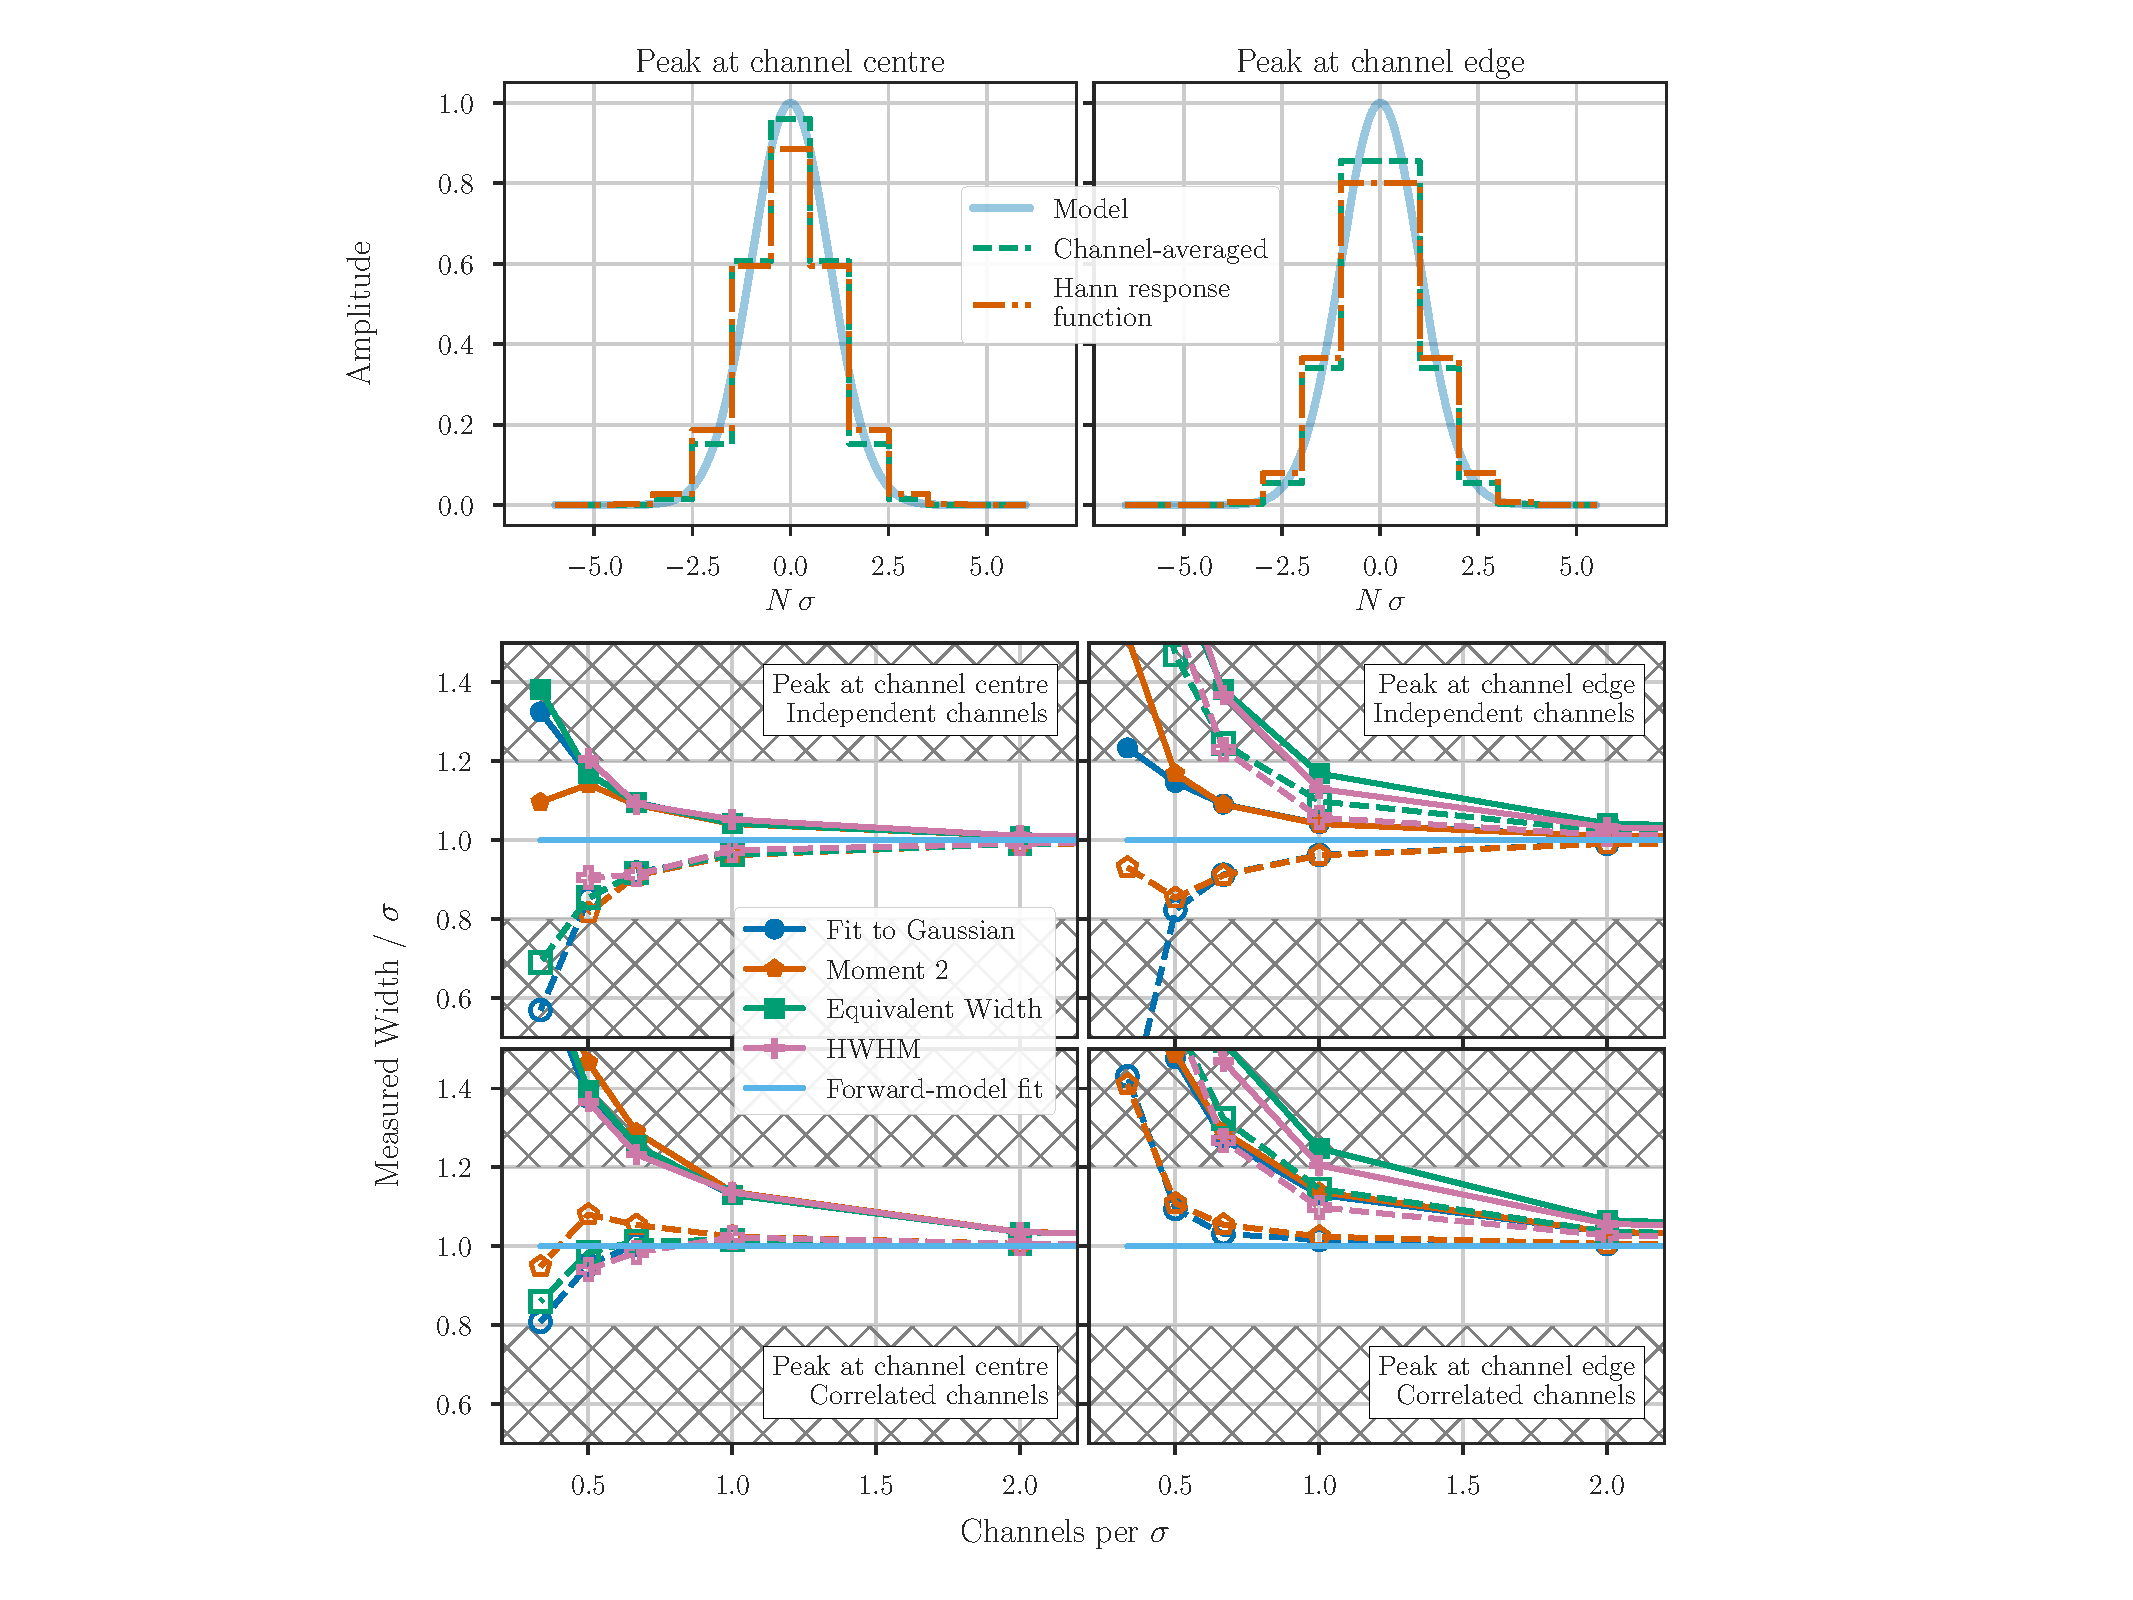
\includegraphics[width=\textwidth]{combined_figure}
\caption{\label{fig:width_recovery_comparison} Comparison of methods for recovering the width of a noiseless Gaussian model as a function of the number of channels per $\sigma$. The first row of panels show a Gaussian sampled with channels of $\Delta v=\sigma$ and how line broadening affects the shape.  The bottom two rows show the line widths measured with different methods, with a correction factor (dashed-unfilled) and without (solid). The middle row is from broadening from channel averaging and the bottom row is convolved with a Hanning response function with $k=0.11$. The first column shows results for a Gaussian at the channel centre and the second column is a Gaussian centred at the channel edge.  Where the peak is located with respect to the channels alters the line broadening.  We find that forward-modelling is the only method that correctly accounts for line broadening in all cases. XXX Change the side labels to independent channels and channels correlated with Hann-like kernel XXX}
\end{figure*}

\acknowledgments

EWK is supported by a Postgraduate Scholarship from the Natural Sciences and Engineering Research Council of Canada (NSERC). EWR acknowledges the support of NSERC (RGPIN-2017-03987).

\software{XXX astropy, numpy, scipy, matplotlib, seaborn XXX}

\begin{thebibliography}{}

\bibitem[Druard et al.(2014)]{druard2014} Druard, C., Braine, J., Schuster, K.~F., et al.\ 2014, \aap, 567, A118.

\bibitem[Heyer et al.(2001)]{heyer2001} Heyer, M.~H., Carpenter, J.~M., \& Snell, R.~L.\ 2001, \apj, 551, 852.

\bibitem[Koch et al.(2018)]{koch2018} Koch, E.~W., Rosolowsky, E.~W., Lockman, F.~J., et al.\ 2018, \mnras, 479, 2505.

\bibitem[Leroy et al.(2016)]{leroy2016} Leroy, A.~K., Hughes, A., Schruba, A., et al.\ 2016, \apj, 831, 16.

\bibitem[Martin et al.(2015)]{martin2015} Martin, T., Drissen, L., \& Joncas, G.\ 2015, Astronomical Data Analysis Software an Systems XXIV (ADASS XXIV), 327.

\bibitem[Rosolowsky, \& Leroy(2006)]{cprops} Rosolowsky, E., \& Leroy, A.\ 2006, Publications of the Astronomical Society of the Pacific, 118, 590.

\bibitem[Rosolowsky et al.(2008)]{rosolowsky2008} Rosolowsky, E.~W., Pineda, J.~E., Foster, J.~B., et al.\ 2008, The Astrophysical Journal Supplement Series, 175, 509.

\bibitem[Stilp et al.(2013a)]{stilp2013a} Stilp, A.~M., Dalcanton, J.~J., Warren, S.~R., et al.\ 2013, \apj, 765, 136.

\bibitem[Stilp et al.(2013b)]{stilp2013b} Stilp, A.~M., Dalcanton, J.~J., Skillman, E., et al.\ 2013, \apj, 773, 88.

\bibitem[Sun et al.(2018)]{sun2018} Sun, J., Leroy, A.~K., Schruba, A., et al.\ 2018, \apj, 860, 172.


\end{thebibliography}

\end{document}
